% Gemini theme
% See: https://rev.cs.uchicago.edu/k4rtik/gemini-uccs
% A fork of https://github.com/anishathalye/gemini

\documentclass[final]{beamer}

% ====================
% Packages
% ====================

\usepackage[size=custom,width=36,height=48,scale=0.5]{beamerposter}
\usetheme{gemini}
\usecolortheme{stanford}
\usepackage{graphicx}
\usepackage{booktabs}
\usepackage{tikz}
\usetikzlibrary{shapes, arrows, positioning}
\usepackage{pgfplots}
\pgfplotsset{compat=1.17}
\usepackage{fontspec}
\usepackage{exscale}
\usepackage{tabularx}
\usepackage{colortbl} % For \rowcolor
\usepackage{xcolor}   % For color definitions
\usepackage{tcolorbox}
\usepackage[backend=biber, style=numeric-comp, maxnames=3, minnames=1, giveninits=true, uniquename=init]{biblatex}
\addbibresource{poster.bib} % Adjust the filename as needed
\usepackage{amssymb}

\setbeamercolor{headline}{bg=cardinalred,fg=white}
\setbeamercolor{footline}{bg=footergray,fg=darkcardinal}

% ====================
% More biblatex kwargs
% ====================

% Remove unnecessary fields
\AtEveryBibitem{
  \clearfield{issn}
  \clearfield{url}
  \clearfield{doi}
  \clearfield{eprint}
  \clearfield{urldate}
}

\AtEveryCitekey{\clearfield{urldate}}

\DeclareFieldFormat{urldate}{}

% Remove "visited on" date
\DefineBibliographyStrings{english}{
  urlseen = {}
}

% Reduce spacing between entries
\setlength{\bibitemsep}{0pt}

% Customize the way certain fields are printed
\DeclareFieldFormat[article]{title}{#1}
\DeclareFieldFormat[article]{volume}{\textbf{#1}}
\DeclareFieldFormat[article]{number}{(#1)}
\DeclareFieldFormat{pages}{#1}

% Customize the order and punctuation of fields
\renewbibmacro*{journal+issuetitle}{%
  \usebibmacro{journal}%
  \setunit*{\addspace}%
  \iffieldundef{series}
    {}
    {\newunit
     \printfield{series}%
     \setunit{\addspace}}%
  \usebibmacro{volume+number+eid}%
  \setunit{\addcolon\space}%
  \usebibmacro{issue+date}%
  \setunit{\addcomma\space}%
  \usebibmacro{issue}%
  \newunit}

\renewbibmacro*{volume+number+eid}{%
  \printfield{volume}%
  \printfield{number}%
  \setunit{\addcomma\space}%
  \printfield{eid}}

% ====================
% Lengths
% ====================

% If you have N columns, choose \sepwidth and \colwidth such that
% (N+1)*\sepwidth + N*\colwidth = \paperwidth
\newlength{\sepwidth}
\newlength{\colwidth}
\setlength{\sepwidth}{0.025\paperwidth}
\setlength{\colwidth}{0.3\paperwidth}

\newcommand{\separatorcolumn}{\begin{column}{\sepwidth}\end{column}}


\title{How Did a Strength-Based Video-Coaching Intervention Alter Parental Neurocognitive Mechanisms? Evidence From RCT \newline Studies in Low-Income, High-Adversity Contexts}


\author{\fontsize{16}{18}\selectfont Howard Chiu \inst{1} \and Nicole Giuliani \inst{2} \and Sihong Liu \inst{3} \and Phil Fisher \inst{3} }

\institute[shortinst]{%
  \inst{1} Graduate School of Education, Stanford University, Stanford, CA, USA \\ 
  \inst{2} College of Education, University of Oregon, Eugene, OR, USA \\ 
  \inst{3} Stanford Center on Early Childhood, Stanford University, Stanford, CA, USA
}

% ====================
% Footer (optional)
% ====================

\footercontent{
  \href{chiuhoward.github.io}{chiuhoward.github.io} \hfill
  Thank you to all the families that made this research possible! \hfill
  \href{mailto:howardchiu@stanford.edu}{howardchiu@stanford.edu}}


% ====================
% Body
% ====================

\begin{document}

% This adds the Logos on the top left and top right
\addtobeamertemplate{headline}{}
{
  \begin{tikzpicture}[remember picture,overlay]
    \node [anchor=north east, inner sep=3cm] at ([xshift=2.25cm,yshift=-2.2cm]current page.north east)
    {
\includegraphics[width=6.25cm]{stanford_logos/GSE-hor-logo-white.png}};
  \end{tikzpicture}

  \begin{tikzpicture}[remember picture,overlay]
    \node [anchor=north east, inner sep=3cm] at ([xshift=18.70cm,yshift=-1.35cm]current page.north east)
    {
\includegraphics[width=36.9cm]{stanford_logos/stanford-line2-10-white.png}};
  \end{tikzpicture}

  \begin{tikzpicture}[remember picture,overlay]
    \node [anchor=north west, inner sep=3cm] at ([xshift=-1.25cm,yshift=-2.2cm]current page.north west)
    {
\includegraphics[width=2.25cm]{osf-qr.png}};
  \end{tikzpicture}
}

\begin{frame}[t]
% Top half - two columns
\begin{columns}[t]
\begin{column}{\textwidth}
  \vspace{-15pt}
  \begin{block}{Filming Interactions to Nurture Development (FIND) Intervention}
    \begin{columns}[t]
      \begin{column}{0.48\textwidth}
          \begin{block}{Parent coaching focuses on Serve and Return interactions}
        \begin{figure}[ht]
          \centering
          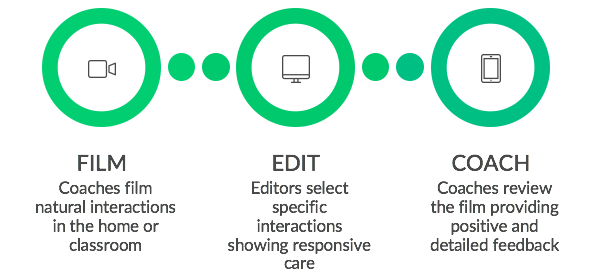
\includegraphics[clip, width=0.75\textwidth]{find.png}
          \label{fig:find}
        \end{figure}
        \vspace{-1cm}
        \begin{figure}[ht]
          \centering
          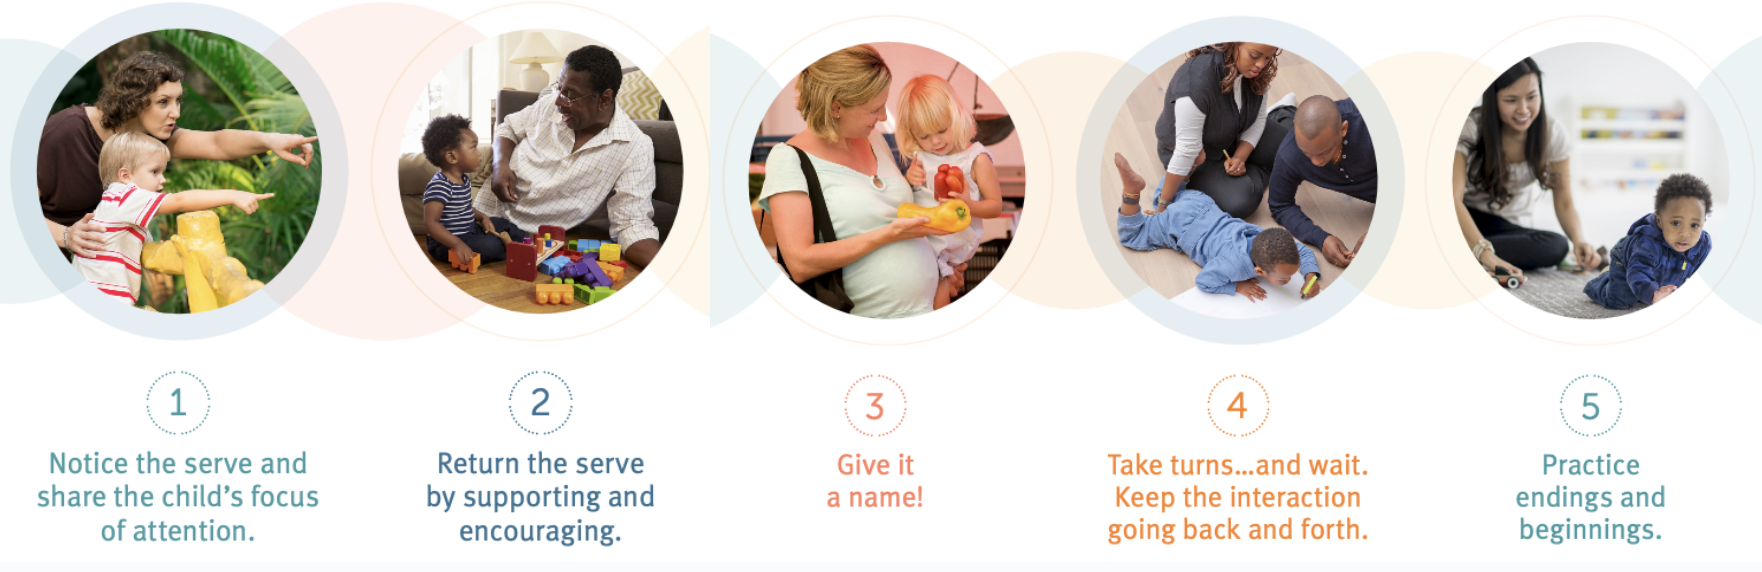
\includegraphics[clip, width=0.85\textwidth]{servereturn.png}
          \label{fig:servereturn}
          \\[0.5em]
          \vspace{-0.5cm}
          {\tiny Source: \url{https://developingchild.harvard.edu/resources/briefs/5-steps-for-brain-building-serve-and-return/}}
        \label{fig:servereturn}
       \end{figure}
             \end{block}
        \vspace{-0.5cm}
        FIND is a 10-session, strengths-based, video-coaching intervention that aims to reinforce naturally occurring, developmentally supportive interactions (known as serve-and-return). FIND has previously been used in homes, child welfare supervised visitation, center- and home-based child care, and pediatric care settings.

      \end{column}

      \begin{column}{0.48\textwidth}

    \begin{block}{Changes in parent brain mediate improvement in child outcomes}
        \begin{figure}[ht]
          \centering
          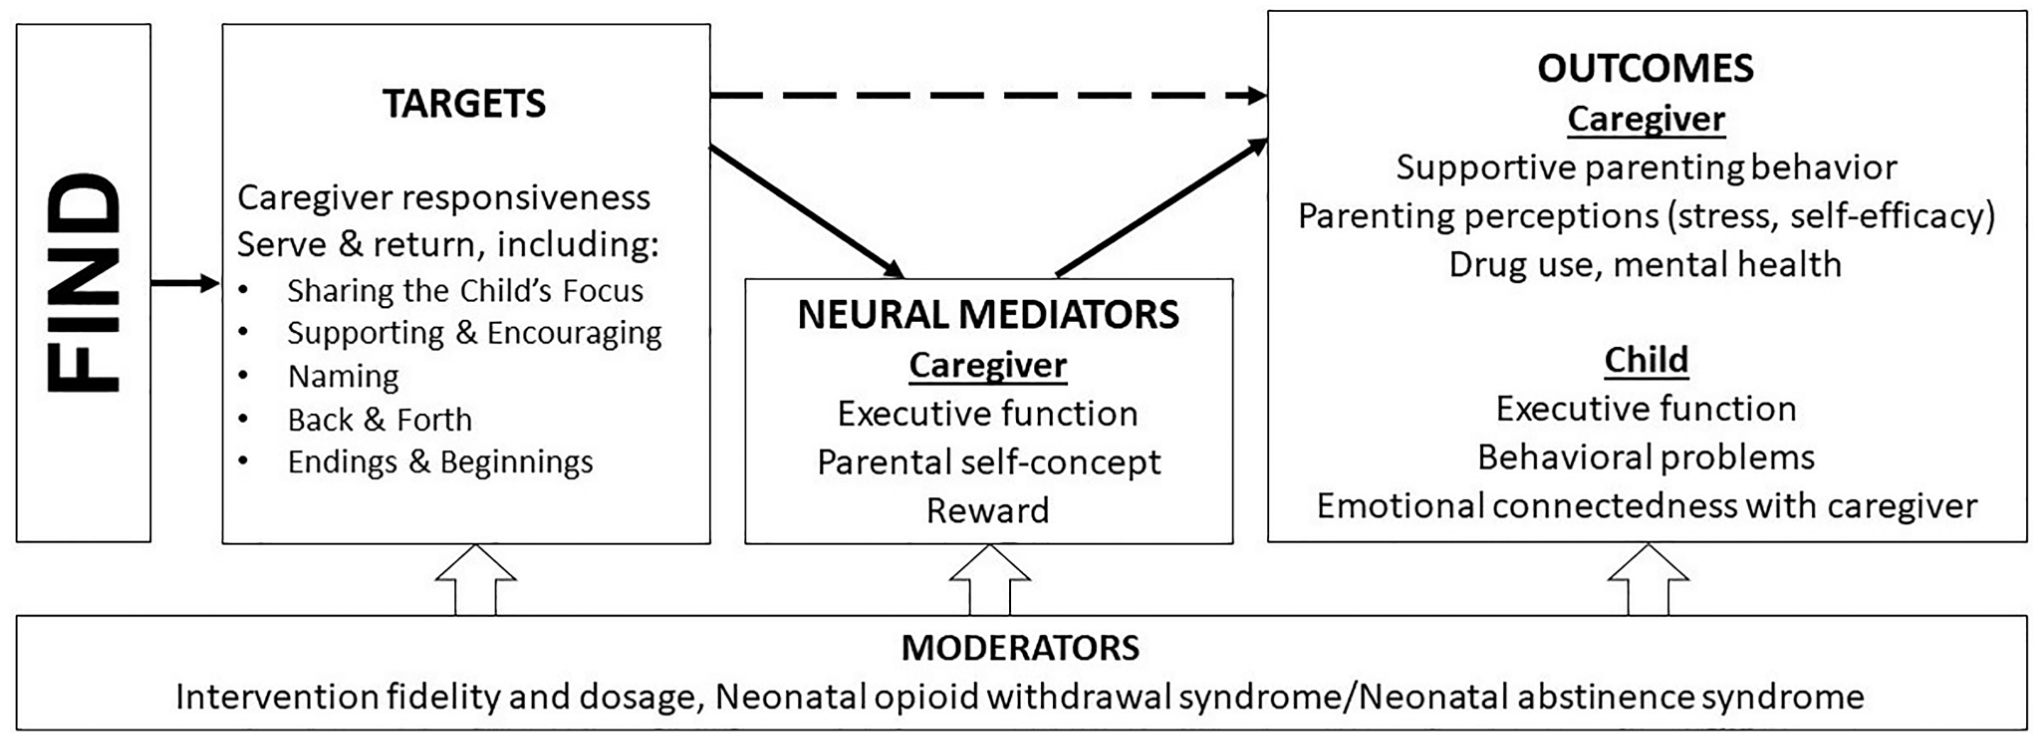
\includegraphics[clip, width=0.75\textwidth]{model.png}
          \label{fig:model}
        \end{figure}
        In earlier studies, FIND led to significant improvements in parent self-efficacy (Liu et al., 2021) and executive function (Giuliani et al., 2019) among middle-income families. 
        Regions of Interest (ROIs) previously identified include clusters in the left inferior frontal gyrus (IFG) and insula for the Correct Stop > Correct Go contrast of the Stop-Signal Task.
        \end{block}

    \begin{block}{Participants included as Intent-to-Treat, but neuroimaging was made optional due to COVID pandemic.}

        \begin{tikzpicture}[node distance=2cm, auto]
            % Define styles
            \tikzstyle{findblock} = [rectangle, draw, fill=cardinalred, 
            text width=4em, text centered, rounded corners, minimum height=3em, font=\small, text=white]
            \tikzstyle{htpblock} = [rectangle, draw, fill=paloaltogreen, 
            text width=4em, text centered, rounded corners, minimum height=3em, font=\small, text=white]
            \tikzstyle{timeline} = [draw, thick, -latex']
            \tikzstyle{wave} = [font=\normalsize, text centered]
            \tikzstyle{label} = [font=\footnotesize, text centered]
            
            % FIND timeline (top)
            \node [findblock] (find_w1) {\textbf{\normalsize n = 55}};
            \node [findblock, right of=find_w1, xshift=2.5cm] (find_w2) {\textbf{\normalsize n = 44}};
            \node [findblock, right of=find_w2, xshift=3.5cm] (find_w3) {\textbf{\normalsize n = 36}};
            
            % HTP timeline (bottom)
            \node [htpblock, below of=find_w1, yshift=0.5cm] (htp_w1) {\textbf{\normalsize n = 59}};
            \node [htpblock, right of=htp_w1, xshift=2.5cm] (htp_w2) {\textbf{\normalsize n = 48}};
            \node [htpblock, right of=htp_w2, xshift=3.5cm] (htp_w3) {\textbf{\normalsize n = 41}};
            
            % Timeline arrows
            \draw [timeline] (find_w1) -- (find_w2) node [midway, above, label, align=center] {\normalsize Intervention \\ \normalsize (10 weeks)};
            \draw [timeline] (find_w2) -- (find_w3) node [midway, above, label] {\normalsize 6 months};
            \draw [timeline] (htp_w1) -- (htp_w2);
            \draw [timeline] (htp_w2) -- (htp_w3);
            
            % Timeline labels
            \node [wave, below of=htp_w1, yshift=1.0cm] {Wave 1};
            \node [wave, below of=htp_w2, yshift=1.0cm] {Wave 2};
            \node [wave, below of=htp_w3, yshift=1.0cm] {Wave 3};
            
            % Group labels
            \node [font=\bfseries, left of=find_w1, xshift=-1.5cm] {FIND};
            \node [font=\bfseries, left of=htp_w1, xshift=-1.5cm, text width=3.4cm, align=center] {HTP \\ (Active Control)};
        
        \end{tikzpicture}

          \end{block}
      \end{column}
    \end{columns}
  \end{block}
\end{column}
\end{columns}

% Bottom half - three columns
\vspace{-0.75cm} % Adjust this value to set the separation between top and bottom halves
\begin{columns}[t]
\separatorcolumn

\begin{column}{\colwidth}
  \begin{block}{FIND improves self-reported parent outcomes (n = 114).}
        
    Consistent with previous pilot and RCT studies, FIND intervention:
    \vspace{-0.3cm}
    \begin{itemize}
        \item reduced parent fatigue post-intervention (time by group effect: B = -1.29, SE = .57, p = .024) and after 6 months (B = -1.35, SE = .60, p = .027)
        \item marginally increased caregiver self-efficacy post-intervention (time by group effect: B = 1.48, SE = .83, p = .076) and after 6 months (B = 1.53, SE = .89, p = .087)
        \item marginally decreased parenting stress after 6 months (B = -2.19, SE = 1.11, p = .051)
    \end{itemize}
    \vspace{-0.5cm}
    \begin{figure}[ht]
        \centering
        \begin{tikzpicture}
            \node[anchor=south west,inner sep=0] (image1) at (0,0) {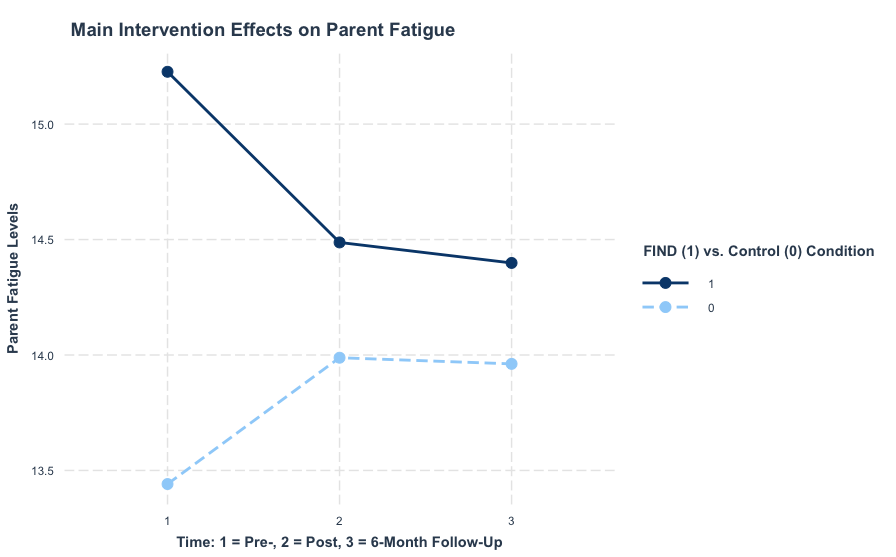
\includegraphics[width=0.625\textwidth]{fatigue.png}};
            \node[anchor=south west,inner sep=0] (image2) at (0.425\textwidth,0cm) {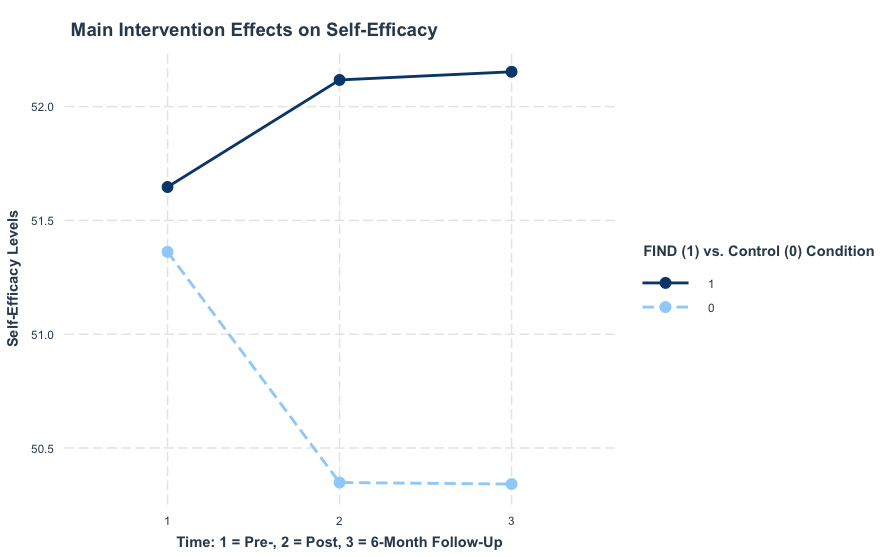
\includegraphics[width=0.625\textwidth]{selfeff.png}};
        \end{tikzpicture}
        {\small FIND intervention effects on parent fatigue (left) and self-efficacy (right); parenting stress not shown.}
        \label{fig:combined}
    \end{figure} 
    
  \end{block}

  \vspace{-0.5cm}

  \begin{block}{References}
    \nocite{*}
    \renewcommand{\bibfont}{\fontsize{8}{10}\selectfont}
    \printbibliography[heading=none]
  \end{block}
\end{column}

\separatorcolumn

\begin{column}{\colwidth}
  
  \begin{block}{FIND had non-significant effects on Parent Self-Evaluation Task (n = 12), behaviorally and in ACC activation.}
    
    \begin{figure}[ht]
      \centering
      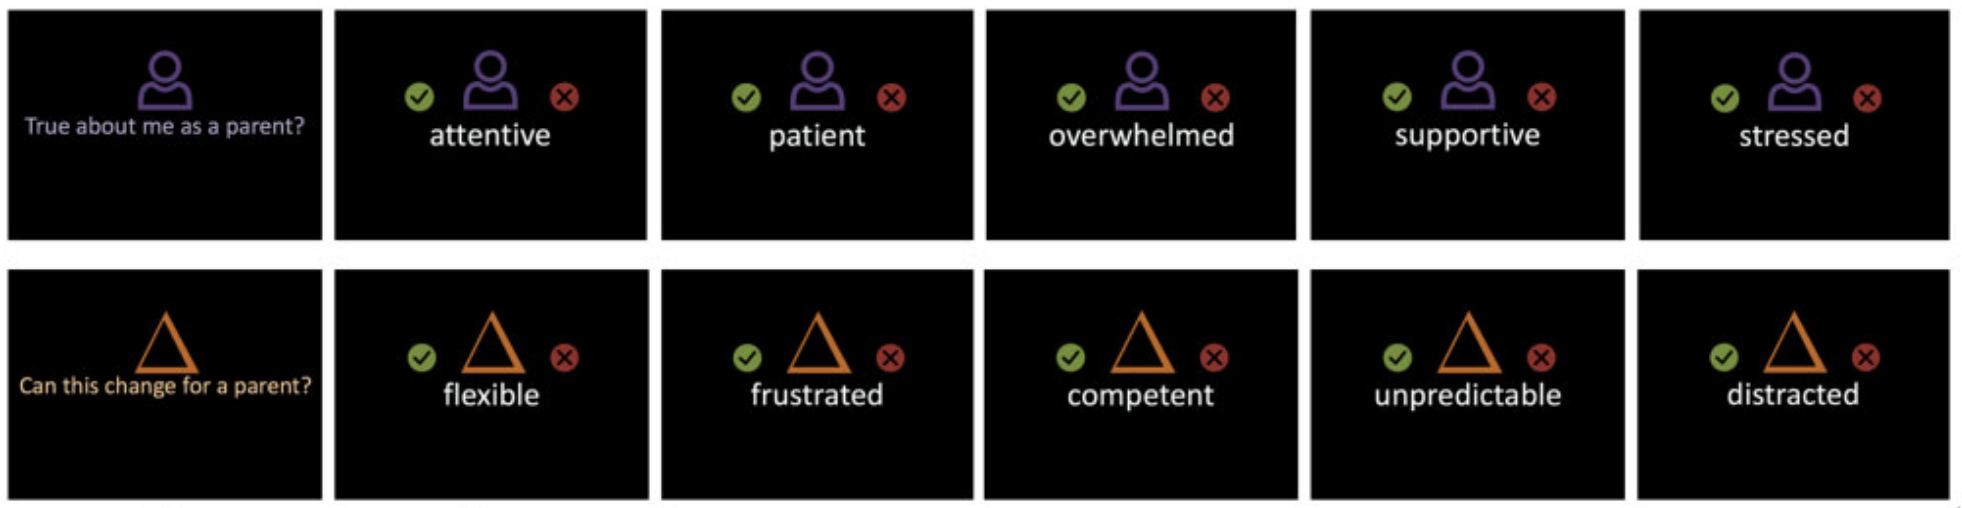
\includegraphics[clip, width=\textwidth]{pset.png}
      \label{fig:pset}
    \end{figure}
    \vspace{-1.0cm}
    \begin{tcolorbox}[colback=paloaltogreen, colframe=paloaltogreen, width=\linewidth]
     \color{white}
     {\text{Endorsement}_{\text{wave2}} = \beta_0 + \beta_1 \text{Endorsement}_{\text{wave1}} + \beta_2 \text{DS} + \beta_3 \text{Self} + \beta_4 \text{FIND} + \epsilon}
    \end{tcolorbox}
    \vspace{-0.2cm}
    \begin{table}[ht]
        \centering
        \fontsize{9}{11}\selectfont
          \begin{tabularx}{\textwidth}{l c c c c}
            \toprule
            \textbf{Parameter} & \textbf{Mean} & \textbf{SD} & \textbf{HDI 3\%} & \textbf{HDI 97\%} \\
            \midrule
            \rowcolor{yellow!50} Endorsement at time 1 & 0.971 & 0.117 & 0.762 & 1.195 \\
            Developmentally Supportive & -0.119 & 5.598 & -10.848 & 10.277 \\
            Statement about Self & 1.965 & 5.387 & -7.721 & 12.446 \\
            FIND condition & -8.024 & 4.305 & -16.355 & -0.265 \\
            \bottomrule
          \end{tabularx}
    \end{table}

    Only proportion of statements endorsed at time 1 significantly predicted proportion of statements at time 2. Adding two and three-way interactions did not improve model fit. No significant differences were observed in the anterior cingulate cortex.

    \vspace{-0.35cm}
    \begin{figure}[ht]
      \centering
      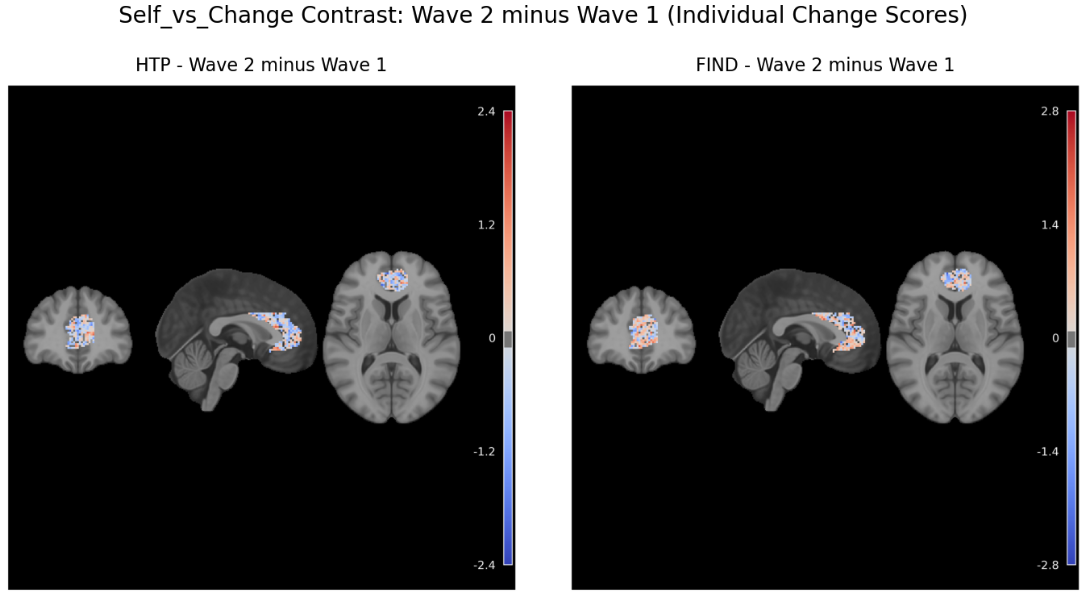
\includegraphics[clip, width=0.75\textwidth]{acc_selfchange.png}
      \label{fig:pset_selfchange}
    \end{figure}
    \vspace{-0.65cm}
    \begin{figure}[ht]
      \centering
      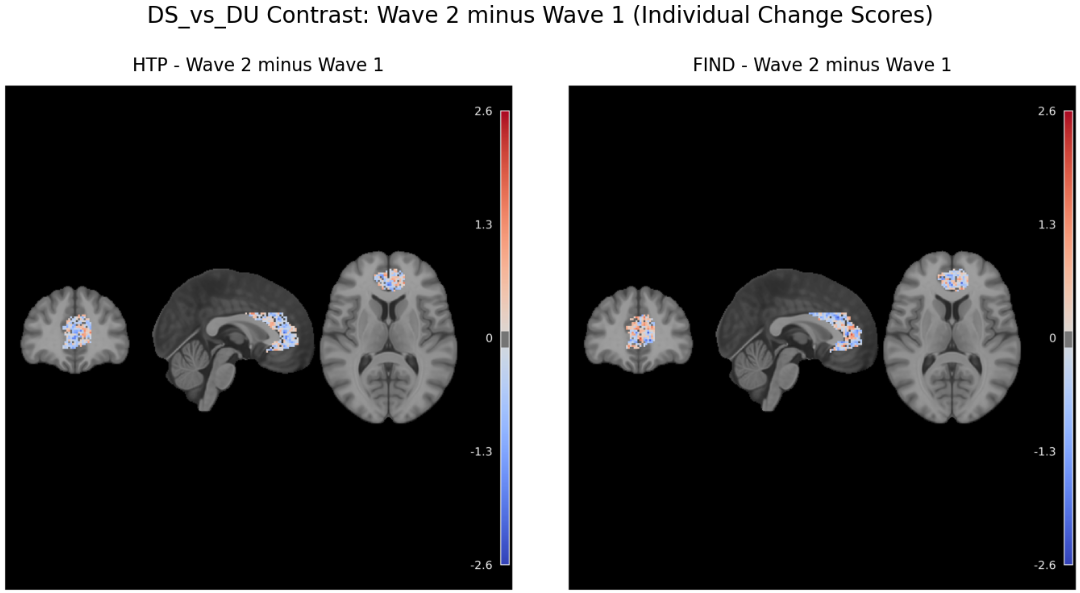
\includegraphics[clip, width=0.75\textwidth]{acc_dsdu.png}
      \label{fig:acc_dsdu}
    \end{figure}
  \end{block}

\end{column}

\separatorcolumn

\begin{column}{\colwidth}
    
      \begin{block}{FIND participants had marginally improved inhibitory control as measured on the Stop Signal Task (n = 17).}

    \begin{figure}[ht]
      \centering
      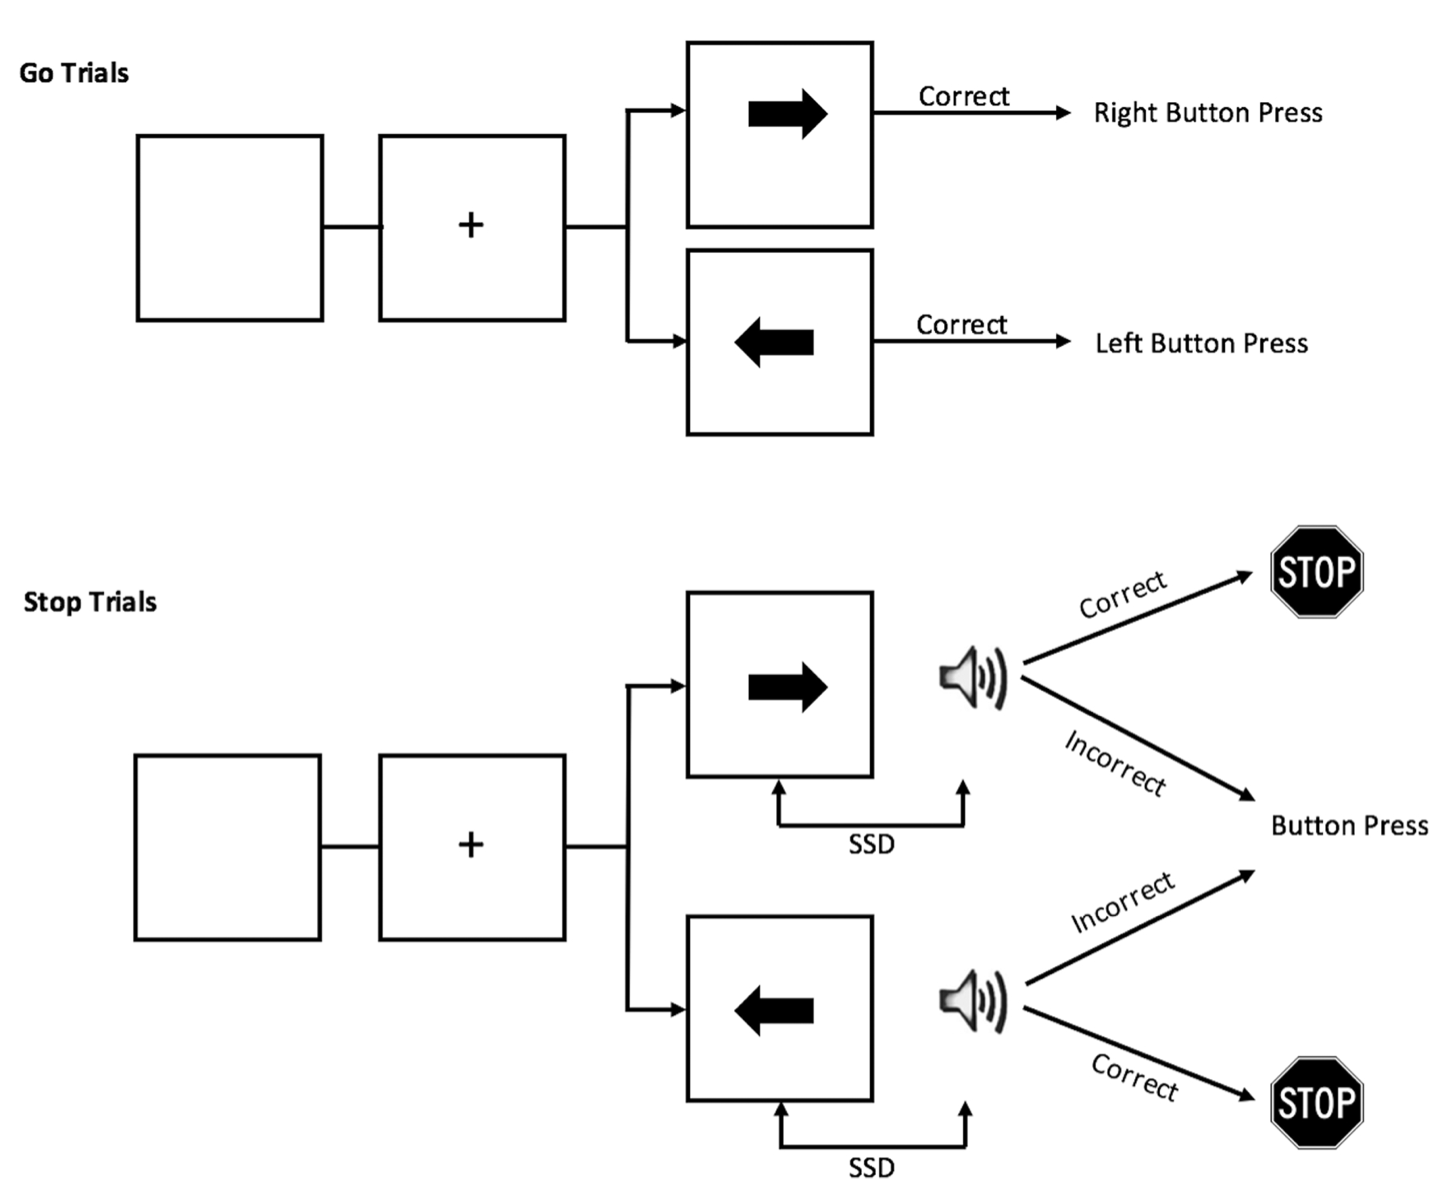
\includegraphics[clip, width=0.6\textwidth]{stopsignal.png}
        \\[0.5em]
        {\tiny Source: Gaillard et al. (2020)}
      \label{fig:stopsignal}
    \end{figure}

    \begin{tcolorbox}[colback=paloaltogreen, colframe=paloaltogreen, width=\linewidth]
     \color{white}
     $\text{SSRT}_{\text{wave2}} = \beta_0 + \beta_1 \text{SSRT}_{\text{wave1}} + \beta_2 \text{FIND} + \epsilon$
    \end{tcolorbox}
    
    \begin{table}[ht]
        \centering
        \fontsize{9}{11}\selectfont
          \begin{tabularx}{\textwidth}{l c c c c}
            \toprule
            \textbf{Parameter} & \textbf{Mean} & \textbf{SD} & \textbf{HDI 3\%} & \textbf{HDI 97\%} \\
            \midrule
            \rowcolor{yellow!50} SSRT at time 1 & 0.720 & 0.254 & 0.242 & 1.190 \\
            FIND condition & -0.050 & 0.026 & -0.097 & 0.001 \\
            \bottomrule
          \end{tabularx}
    \end{table}

    SSRT at time 2 was mainly predicted by SSRT at time 1 rather than intervention condition. Adding a two-way interaction did not improve model fit. We will be analyzing the neuroimaging data soon.
    
  \end{block}
    \vspace{-0.5cm}

    \begin{figure}[ht]
        \centering
          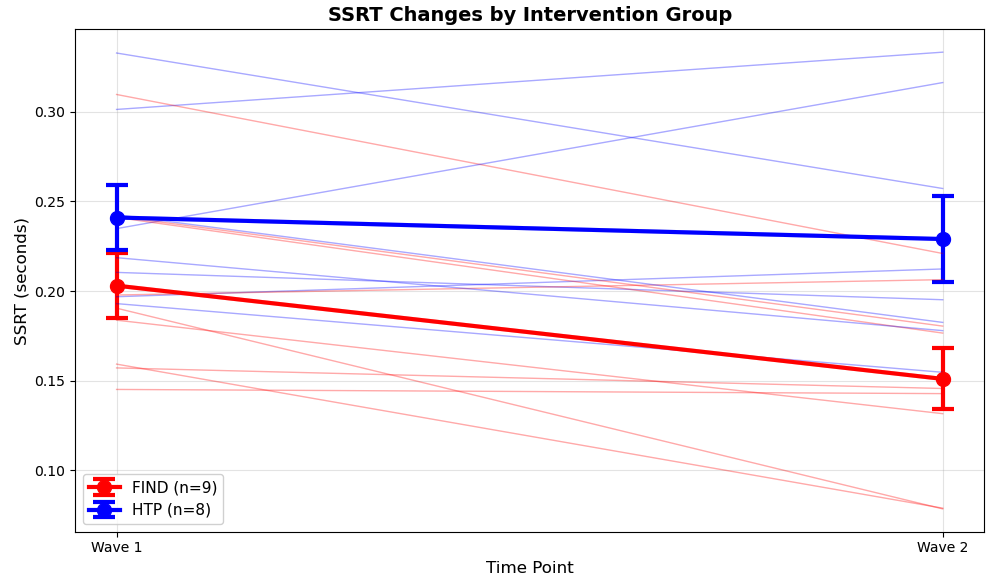
\includegraphics[clip, width=\textwidth]{ssrt.png}
          \label{fig:ssrt}
    \end{figure}

\end{column}

\separatorcolumn
\end{columns}
\end{frame}

\end{document}